\documentclass[11pt]{article}

% Package for better formatting of the mathematics
\usepackage{amsmath, amsthm, amssymb, amsfonts}

% For better handling of figures and placements
\usepackage{graphicx}

% Define theorem styles
\newtheorem{theorem}{Theorem}
\newtheorem{lemma}[theorem]{Lemma}
\newtheorem{forklaring}[theorem]{Forklaring}
\newtheorem{proposition}[theorem]{Proposition}
\newtheorem{corollary}[theorem]{Corollary}

\theoremstyle{definition}
\newtheorem{definition}{Definition}
\newtheorem{example}{Example}
\newtheorem{exercise}{Exercise}

\theoremstyle{remark}
\newtheorem*{remark}{Remark}
\newtheorem*{note}{Note}

\title{Algoritmer og Sandsynlighed \\ \large Kompendium}

\author{Kevin Vinther}

\begin{document}

\maketitle
\tableofcontents

\newpage


\section{Basic Counting Problems}
\label{sec:basiccounting}


\section{Inclusion Exclusion}
\label{sec:inclexcl}


\section{Discrete Probability}
\label{sec:discprob}


\section{Randomized Algorithms}
\label{sec:random}

\section{Probabilistic Analysis}
\label{sec:proban}

\section{Indicator Random Variables}
\label{sec:indicator}

\section{Universal Hashing}
\label{sec:hashing}

\section{String Matching}
\label{sec:string}

\subsection{Notation}
\label{subsec:stringnotation}

Jeg tænker ikke at der skal snakkes om det her til eksamen, men følgende er en liste af notation der er nødvendige for  forforståelse:

\begin{itemize}
\item \textbf{Strenge}: Arrays med karakterer (ligesom i programmeringssprog)
\item \textbf{Shift}: Hvor langt inde i en streng
\item $P[1..m]$: Mønster med længde $m$
\item $T[1..n]$: Tekst med længde $n$
\item $T[1..n-m]$: Den tekst vi leder efter. Vi er ikke interesseret i de sidste $m$, da de er længere end mønsterstrengen.
\item \textbf{P forekommer med shift s}: Du finder mønstret $s$ karakterer inde i teksten.
\item \textbf{Validt shift} et shift hvor mønsteret $P$ forekommer
\item \textbf{Invalidt shift} et shift hvor mønsteret $P$ \textbf{ikke} forekommer. 
\end{itemize}
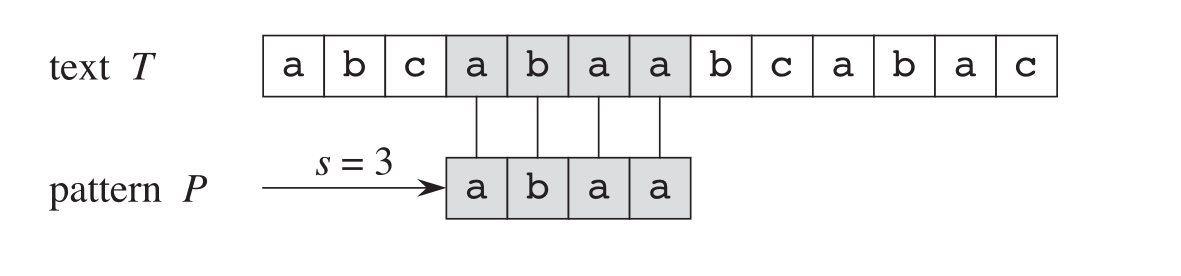
\includegraphics[width=400pt]{main--string-matching--notation-81a7.png}

\begin{itemize}
\item $\Sigma^{*}$ (Sigma-Stjerne) er sættet af alle endelige strenge der kan bliver lavet fra karaktererne i $\Sigma$. 
\item $\varepsilon$, den \textbf{tomme streng}, er strengen uden noget indhold. Den er også en del af $\Sigma^{*}$.
\item $|x|$ er længden af streng $x$. 
\item \textbf{Concatenation} af to strenge $x$ og $y$, skrevet $xy$ har længde $|x| + |y|$ og er karaktererne i $x$ efterfulgt af karaktererne i $y$.
\item \textbf{Præfiks} af streng $x$, denoted $w \sqsubset x$, gælder hvis $x = wy$ hvor $y \in \Sigma^{*}$, altså, $w$ er en del af streng $x$ i starten af strængen. $y$ er den resterende del af streng $x$, som ikke er $w$.
\item \textbf{Suffiks}: denoted $w \sqsupset x$ omvendt. 
\end{itemize}

\begin{lemma}[31.1 (Overlapping-suffix lemma) (Cormen)]
Suppose that $x,y$, and $z$ are strings such that $x \sqsupset z$ and $y \sqsupset z$. If $|x| \leq |y|$, then $x \sqsupset y$. If $|x| \geq |y|$, then $y \sqsupset x$. If $|x| = |y|$ then $x = y$.
\end{lemma}

\begin{proof}
  Se Figur ~\ref{fig:overlappingsuffix}
\end{proof}

\begin{figure}[ht]
  \centering
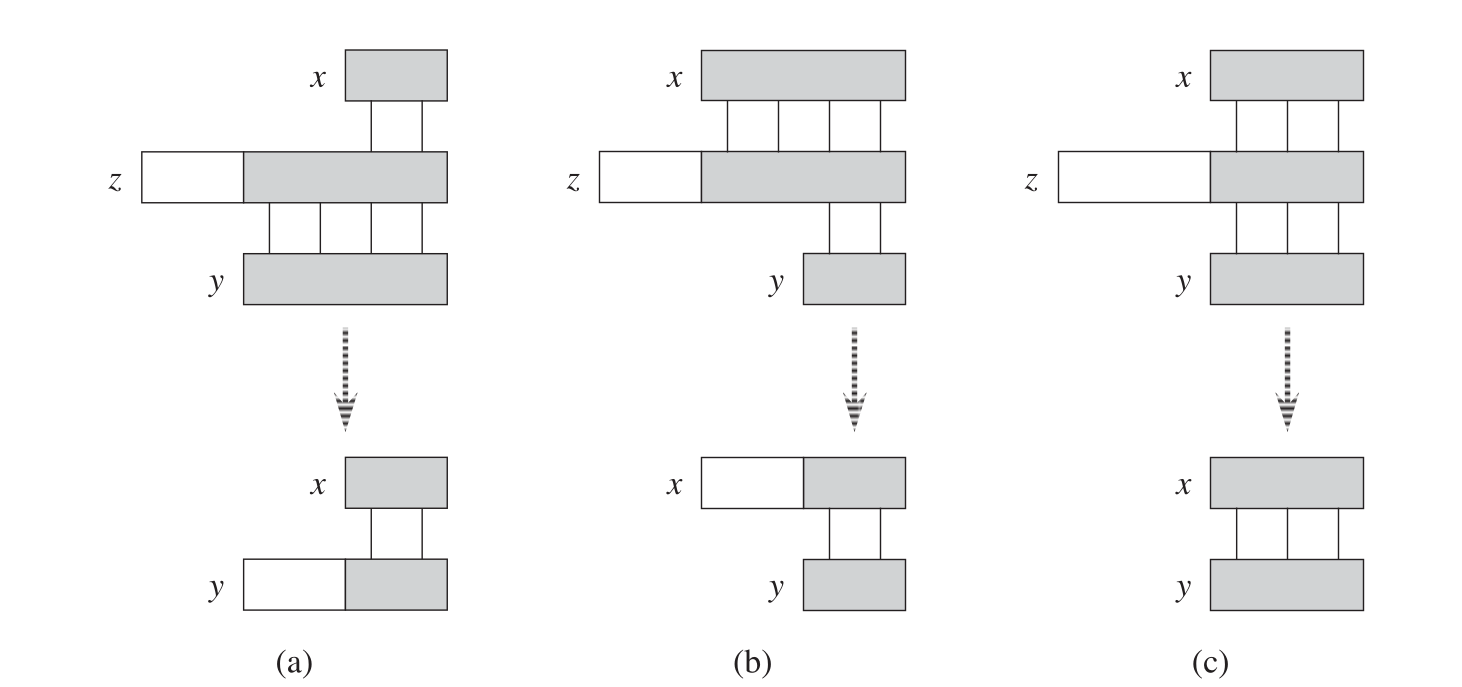
\includegraphics[width=400pt]{main--string-matching--notation-1e22.png}
  \caption{\label{fig:overlappingsuffix} Vi antager at $x \sqsupset z$ og $y \sqsupset z$. De tre dele af figuren illustrerer de tre cases af lemmaet. \textbf{(a)} Hvis $|x| \leq |y|$, så $x \sqsupset y$. \textbf{(b)} Hvis $|x| \geq |y|$, så $y \sqsupset x$. \textbf{(c)} Hvis $|x| = |y|$, så er $x = y$.}
\end{figure}

Vi antager at tiden det tager for at finde ligheden mellem to strenge er $\Theta(t+1)$ hvor $t$ er størrelsen af den længste streng. $+1$, til hvis $t = 0$.



\subsubsection{Køretids Overview}

\begin{table}[h]
\begin{tabular}{|l|l|l|}
\hline
\textbf{Algorithm}          & \textbf{Preprocessing Time} & \textbf{Matching Time} \\ \hline
\textit{Naive}              & $0$                         & $O((n-m+1)m)$          \\ \hline
\textit{Rabin-Karp}         & $\Theta (m)$                & $O((n-m+1)m)$          \\ \hline
\textit{Finite Automaton}   & $O(m |\Sigma |)$            & $\Theta (n) $          \\ \hline
\textit{Knuth-Morris-Pratt} & $\Theta (m)$                & $\Theta (n)$           \\ \hline
\end{tabular}
\end{table}


\subsection{Naive Algoritme}
\label{subsec:naive}

\begin{itemize}
\item Hvad er den? 
\item Hvorfor er den dårlig? 
\item Hvad er worst-case? 
\end{itemize}


Den naive algoritme er virkelig det, naiv.
\textbf{Source Code}:

\begin{verbatim}
Naive-String-Matcher(T,P)
n = T.length
m = P.length
for s = 0 to n - m
    if P[1..m] == T[s+1..s+m]
        print "Pattern occurs with shift " s
\end{verbatim}

\subsubsection{Køretid}

Den er virkelig skrald. Køretiden er $O((n-m+1)m)$. Dens worst case sker hvis teksten er $a^{n}$ og mønsteret der ledes efter er $a^{n}$ (begge er mængder af $a$'er, på længde hhv. $m$ og $n$. I dette tilfælde finder den matches hver gnag, og der tager dermed $O(n^{2})$ tid.

Der er \textbf{ingen} preprocessing tid, da der ikke skal gøres noget før algoritmen kører.



\subsection{Rabin-Karp}
\label{subsec:rabinkarp}

\begin{itemize}
\item Hvad er hovedidéen? 
\item Hvorfor er den bedre end naive? 
\end{itemize}

Trods at Rabin-Karp har en worst-case køretid på $\Theta((n-m+1)m)$ er dens gennemsnitlige køretid bedre.

Algoritmen konverterer bogstaverne til tal, i radix-$d$ notation, hvor $d$ er størrelsen på alfabetet, $|\Sigma|$.

I følgende eksempler vil vi gå ud fra at $d = 10$, og $\Sigma = \{0, 1, \ldots, 9\}$. Husk at $P[1..m]$ er mønsteret vi leder efter. Ved rabin-karp skelner vi mellem $P[1..m]$ og $p$, hvor $p$ er dets decimalværdi. Dvs., hvis $P[1..m] = 1372$, så er $p = 1372$ i decimalværdi. Eksemplet virker forsimplet idet vores alfabet også er tal, men tænk hvis alfabetet var $\Sigma = \{a, b, ... j\}$, i dette tilfælde ville $p$ ikke være ændret, men $P[1..m] = acgb$. Ydermere er teksten $T[1..n]$'s decimal counterpat $t_{s}$. Den bliver udregnet på samme måde. Hvis $t_{s} = p$ så $T[s+1..s+m] = P[1..m]$.

Vi vil gerne have en måde hvorpå vi kan lave alfabetet om til tal, som vi kan regne på. Hvis vi kan konverterer mønsteret $P[1..m]$ til $p$ på $\Theta(m)$ tid, så kan vi konvertere $t_{s}$ på $\Theta(n-m+1)$ tid. Til at gøre dette bruger vi \textbf{Horner's Rule}, som er meget vigtig at kende, se Definition ~\ref{def:horner}.

\begin{definition}[Horner's Rule]
  \label{def:horner}
  Horner's Rule er en regel hvorpå du hurtigt (specielt for computere) kan udregne decimaltal. Dette gør du ved at tage det sidste tal der skal udregnes først, derefter tager du tallet på 10'ernes plads, ganger det med $10^{1}$, etc. indtil du er ved $d$'ende plads, og ganger det med $10^{d}$\footnote{Dette gælder kun i base-10. Rabin-karp kører i base-b. Konverter dette til $b^{d}$}. Se følgende billede.


    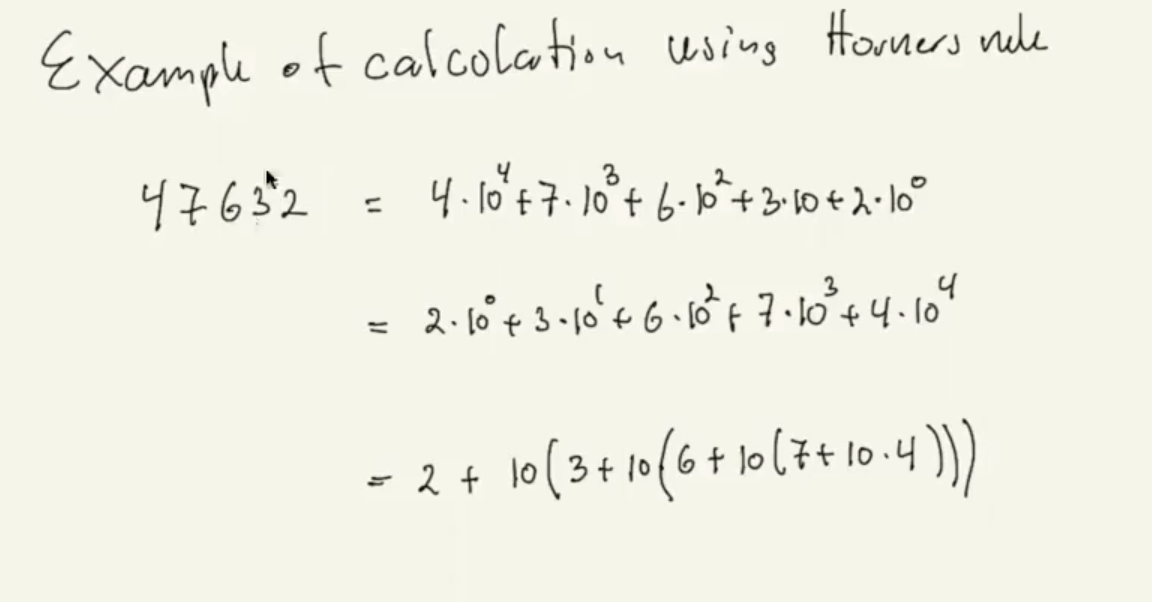
\includegraphics[width=300pt]{../Question8/main--the-naive-string-matching-algorithm--rabin-karp-c553.png} 
\end{definition}

Noget af det smarteste med Horner's Rule, er at, når du går til næste værdi, så kan du udregne det hurtigt uden at tage det hele om igen. Dette giver køretid $\Theta(n-m)$:

\[ t_{s+1} = 10(t_{s} - 10^{m-1}T[s+1]) + T[s+m+1] \]


\begin{forklaring}
\textit{Skip dette hvis du ikke har meget tid.} $10^{m-1} \cdot T[s+1]$ fjerner det højeste ciffer. Ved at gange det med 10 skifter du tallet til venstre med en cifferposition. Ved at tilføje $T[s+m+1]$ får du det nye, laveste ciffer. 
\end{forklaring}

\textbf{Problem!} $p$ og $t_{s}$ er muligvis for storre til at de kan være i et computer \texttt{word}. Hvis dette er tilfældet, og $P$ indeholder $m$ karakterer, så tager vi tallet \textbf{modulo }$q$. $p \mod q$ bliver udregnet på $\Theta(m)$ tid (størrelsen af $p$.) Alle $t_{s}$ værdier i $\Theta(n-m+1)$ tid.

\textbf{Hvilken $q$ skal vi dog vælge?} Simpelt! Vælg et primtal således der er plads til $10q$  i én computer \texttt{word}. Derefter kan vi udføre alle udregninger simpelt. Ved at bruge modulo-udregning, ændrer Horner's udregning sig til at blive: $t_{s+1} = (d(t_{s} - T[s+1]h) + T[s+m+1]) \mod q$, hvor $h \equiv d^{m-1} (\mod q)$ er værdien af ciffret $1$ i højeste position. 

\textbf{Problem igen!} Hvad hvis $p \equiv t_{s}$, men $P[1..m] \neq T[s+1..n-m]$? Altså, tallene er ens, men de er strengene ikke grundet modulo? Dette kalder vi et \textbf{spurious hit}, og er pisse irriterende, men desværre end nødvendig onde. Derfor, når vi finder et \textbf{hit} om det er spurious eller ej, så tjekker vi også strengene. 

\begin{figure}[ht]
  \centering
  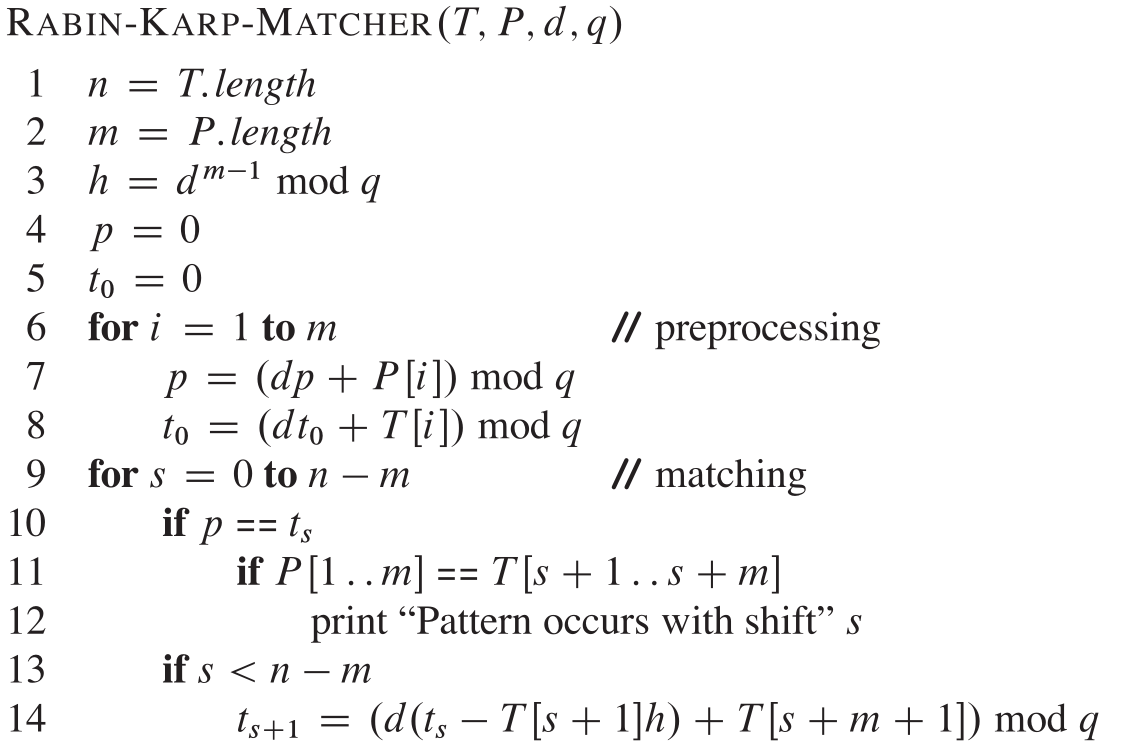
\includegraphics[width=400pt]{main--string-matching--rabin-karp-9fe7.png}
  \caption{\label{fig:rabinkarpalgorithm} Rabin Karp Algoritmen}
\end{figure}


Worst-case er i samme situation som ved den naive algoritme. Hvis teksten er en del a'er, og det samme med mønstret, så vil vi få en masse hits.






\subsection{Finite Automaton Based}
\label{subsec:DFA}

\begin{itemize}
\item Hvordan laver man en DFA?
\end{itemize}






\section{Flows}
\label{sec:flows}

\section{Min-Cut}
\label{sec:mincut}





\end{document}
